\documentclass[a4paper]{article}

\renewcommand{\familydefault}{\sfdefault}
\usepackage{xcolor}
\usepackage{tcolorbox} 
\usepackage{sectsty}
\usepackage{graphicx}
\usepackage{enumitem} 
\usepackage{calc}
\usepackage{circuitikz}
\usepackage[ngerman]{babel}
\usepackage{latexsym,amssymb,amsmath}
\usepackage{pdfpages}
\usepackage{siunitx}

\sectionfont{\fontsize{12}{15}\selectfont}

\definecolor{myred}{HTML}{f03e3e}
\definecolor{myblue}{HTML}{1c7ed6}

\newcommand{\complex}[1]{\underline{#1}}

\newcommand{\mumlaut}[1]{\text{\textit{\"#1}}}
\newcommand{\uev}[1]{\textcolor{myred}{\mumlaut{#1}}}

\begin{document}

\begin{center}
  \Large Das einphasige Ersatzschaltbild des Drehstromtransformators, Teil 2
\end{center}

\begin{flushright}
  R.G., 2020
\end{flushright}

\section{Vereinfachung des Ersatzschaltbildes des Drehstromtransformators}

    \begin{center}
      \begin{circuitikz}[european, scale = 0.8]
        \node (inputA) at (0,0) {};
        \node (inputB) at (0,-3) {};

        \node (outputA) at (12, 0) {};
        \node (outputB) at (12, -3) {};

        \draw (inputA) to[R, l=$R_{1}$, i=$\complex{I_{1}}$, o-] (3,0);
        \draw (3,0) to [L, l=$L_{1} - M'$] (6,0);
        \draw (6,0) to [L, l=$M'$, *-*] (6,-3);
        \draw (6,0) to [L, l=$L_{2}' - M'$] (9,0);
        \draw (9,0) to [R, l=$R_{2}'$, i=$\complex{I_{2}'}$, -o] (outputA);

        \draw (inputB) to[short, o-o] (outputB);

        \draw (inputA)  to[open, v=$\complex{U_{1}}$] (inputB);
        \draw (outputA) to[open, v^=$\complex{U_{2}}'$] (outputB);

        \draw (3,-1.5) node[scale=4, color=lightgray]{$\circlearrowright$};
        \draw (3,-1.5) node[color=lightgray]{$(11)$};

        \draw (9,-1.5) node[scale=4, color=lightgray]{$\circlearrowright$};
        \draw (9,-1.5) node[color=lightgray]{$(12)$};

      \end{circuitikz}
    \end{center}

Für den \textbf{belasteten} Transformator gilt folgende Überlegung: Die hochohmige Quergröße $X_{n}'$ ($M'$) führt gegenüber den Lastströmen einen vernachlässigbar geringen Strom. Daraus ergibt sich folgende Vereinfachung:

\[X_{n} \rightarrow \infty\]

\noindent Es ergibt sich nun die Reihenschaltung, welche als $Z_{T}$ definiert wird:
\[ Z_{T} = R_{1} + j X_{1} + R2' + j X_{2}'\]


\begin{center}
    \begin{circuitikz}[european]
        \draw (0,0) to[R, l=$Z_{T}$, i = $I'$, o-o] (4,0);
        \draw (4,-2) to[short, o-o] (0, -2);
        \draw (0,0) to[open, v=$U_{1}$] (0,-2);
        \draw (4,0) to[open, v^=$U_{2}'$] (4,-2);
    \end{circuitikz}
\end{center}

Nicht eingezeichnet ist der ideale Übertrager mit ü sowie $\complex{I}$ und $\complex{U_{2}}$ am Ausgang.\\

Auf dem Typenschild des Transformators steht die relative, d.h. auf die Nennspannung bezogene, Kurzschlussspannung $u_{k}$. Wie man daraus die Transformatorimpedanz berechnet ist unten gezeigt.


\section{Typenschild eines Dreiphasentransformators}
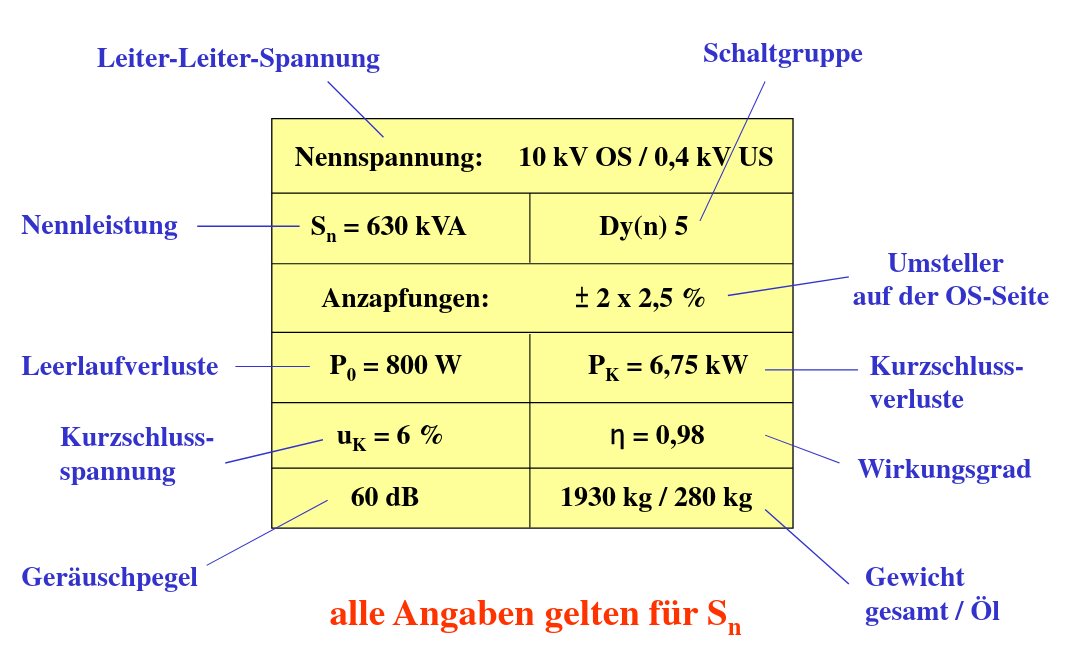
\includegraphics[width = \textwidth]{typenschild.png}

\subsection{Leiter-Leiter-Spannung $U_{n}$}
Die Nennspannung wird angegeben für Ober- und Unterspannungsseite als Leiter-Leiter-Spannung. Wir bezeichnen sie als $U_{n}$.

\subsection{Nennleistung $S_{n}$}
Die Nennleistung $S_{n}$ definiert u.a. den Nennbetrieb des Transformators.

\subsection{Schaltgruppe}
Die Schaltgruppe gibt an, wie jeweils Ober- und Unterspannungsseite des Transformators mit dem Dreiphasennetz verschaltet werden.\\

\subsubsection{Kennzeichnung}
\noindent Die Kennzeichnung setzt sich wie folgt zusammen:
\begin{enumerate}
    \item Schaltungsweise der Oberspannungsseite (Großbuchstabe)
    \item Schaltungsweise der Unterspannungsseite (Kleinbuchstabe)
    \item Stundenzahl (Uhr) als Angabe der Phasenverschiebung zwischen den Leiter-Leiter-Spannungen, Phase 1 steht auf 12 Uhr
\end{enumerate}

\subsubsection{Mögliche Schaltungsarten}
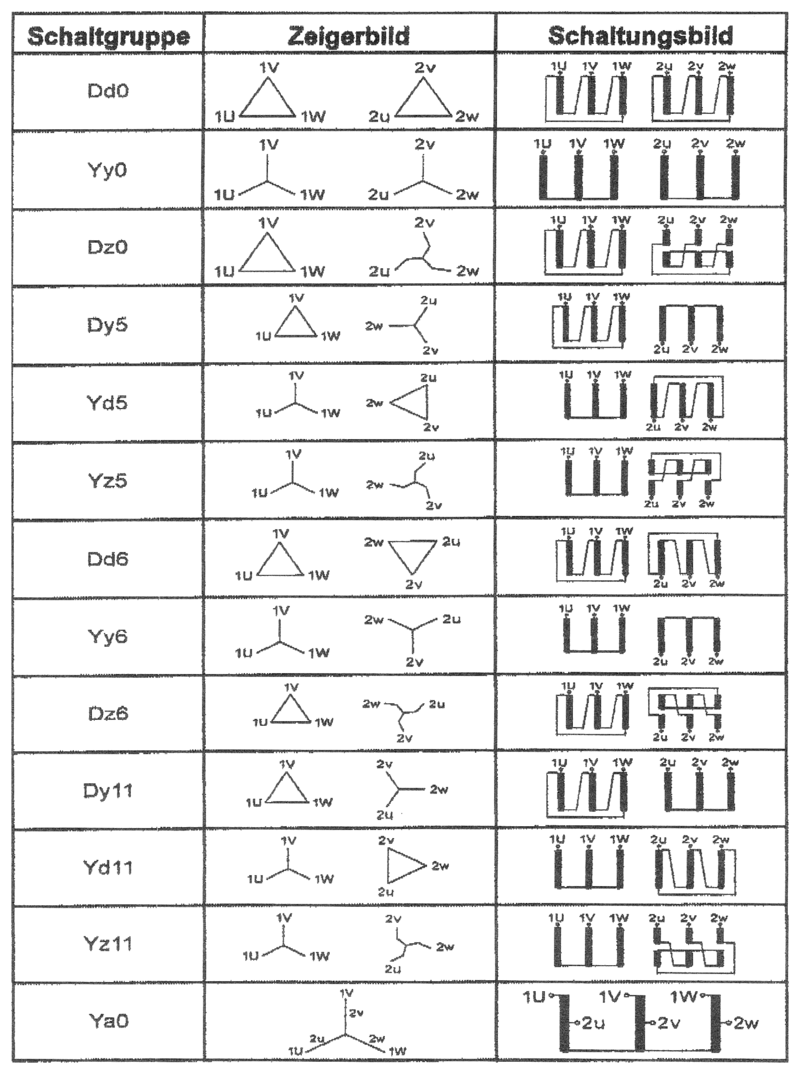
\includegraphics[width=\textwidth]{Schaltgruppe-Zeigerbild.png}

\subsection{Leerlaufverluste $P_{0}$}
$P_{0}$ sind die Verluste bei Leerlauf des Transformators, d.h. wenn er auf der Sekundärseite nicht belastet wird (offen).

\subsection{Kurzschlussverluste $P_{k}$}
$P_{k}$ sind die Verluste bei Kurzschluss des Transformators, d.h. wenn er maximal belastet wird.

\subsection{Kurzschlussspannung(sfaktor) $u_{k}$}
Auf dem Typenschild wird $u_{k}$ angegeben als Bruchteil der Nennspannung $U_{n}$ im Kurzschlussfall (z.B. $6 \si{\percent}$).

\subsection{Wirkungsgrad $\eta$}
$\eta$ ist der Wirkungsgrad des Transformators, also das Verhältnis von abgegebener zu aufgenommener Wirkleistung.

\subsection{Geräuschpegel}
Der Geräuschpegel wird in $\text{dB SPL}$ angegeben. Er entsteht z.B. durch \emph{Magnetostriktion}.

\section{Kenngrößen des vereinfachten Ersatzschaltbildes}

\begin{center}
    \begin{circuitikz}[european]
        \draw (0,0) to[R, l=$Z_{T}$, o-] (4,0);
        \draw (4,0) to[short, i=$I_{n}$] (4, -2);
        \draw (4,-2) to[short, -o] (0, -2);

        \draw (0,0) to[open, v=$U_{K}$] (0,-2);
      \end{circuitikz}

      \[U_{K} ... \text{Kurzschlussspannung}\]

\end{center}

\begin{enumerate}
    \item Einfacher Strom-Spannungs-Zusammenhang:
    \[Z_{T} = \frac{U_{K}}{I_{n}}\]
    \item Zusammenhang des Kurzschlussfaktors $u_{k}$ ($U_{K}$ - Strangspannung!):
    \[u_{k} = \frac{U_{K}}{U_{n} / \sqrt{3}}\] z.B $6 \si{\percent}$
    \item Zusammenhang der Nennscheinleistung:
    \[S_{n} = {\color{gray}\underbrace{\color{black}\sqrt{3}}_{\text{in allen 3 Phasen}}} \cdot {\color{gray}{\underbrace{\color{black}U_{n}}_{\text{Leiter-Leiter-Spannung}}}} \cdot {\color{gray}\underbrace{\color{black}I_{n}}_{\text{Strangstrom}}}\]

  \item Einsetzen in Gleichung der Transformatorimpedanz (Betrag):
    \[Z_{T} = \frac{u_{k} \cdot U_{n}^{2}}{S_{n}}\]

  \item Wicklungsverluste:
    \[P_{Kn} = 3 \cdot I_{n}^{2} \cdot R_{T}\]
    \[\frac{P_{K}}{P_{Kn}} = \frac{3 \cdot I^{2} \cdot R_{T}}{3 \cdot I_{n}^{2}\cdot R_{T}} = (\frac{I}{I_{n}})^{2}\]

    \[P_{V} = P_{0} + P_{K}\]

\end{enumerate}

\section{Übung: Belasteter Drehstromtransformator}



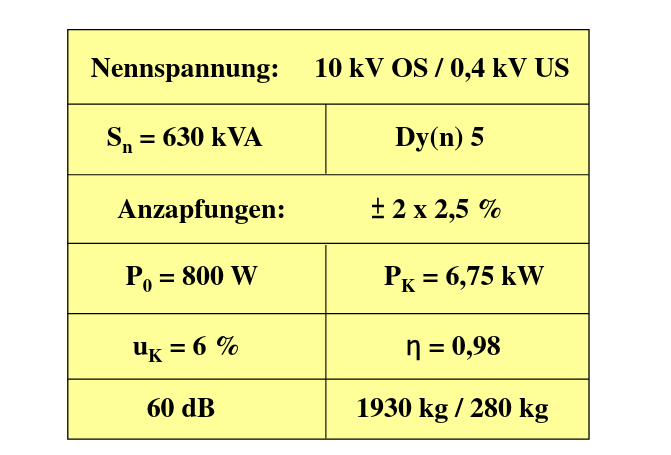
\includegraphics[width=\textwidth]{uebung.png}
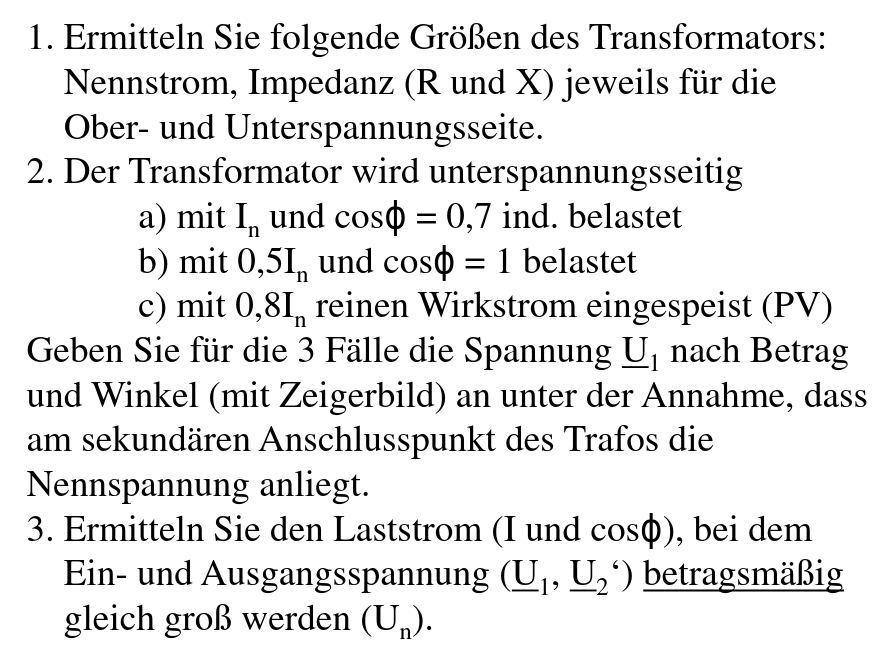
\includegraphics[width=\textwidth]{aufgaben.png}

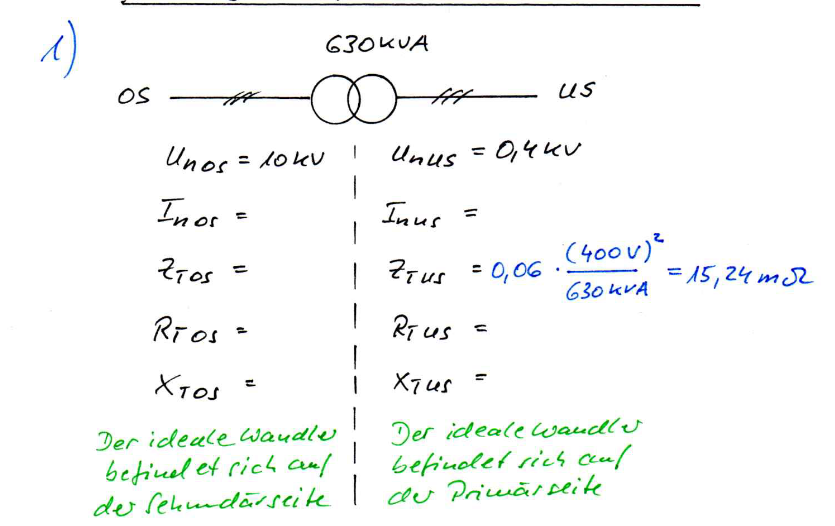
\includegraphics[width=\textwidth]{uebtab.png}
\subsection{}
\subsubsection{Oberspannungsseite}
\begin{enumerate}
    \item Nennstrom:
    \[S_{n} = \sqrt{3} \cdot U_{nOS} \cdot I_{n}\]
    \[I_{n} = \frac{S_{n}}{\sqrt{3}U_{nOS}} = 36.37 \, \si{\ampere} \]


    \item Impedanz (idealer Übertrager auf Sekundärseite)
    \[Z_{T_{OS}} = \frac{U_{nOS}^{2} \cdot u_{k}}{S_{n}} = 9.52 \, \si{\ohm}\]

    \item Resistanz aus den Wirkleistungsverlusten bei KURZSCHLUSS
    \[R_{T_{OS}} = \frac{1}{3} \cdot \frac{P_{K}}{I_{nOS}^{2}} = 1.7 \, \si{\ohm}\]

    \item Reaktanz aus dem Betrag der Impedanz
    \[X_{T_{OS}} = \sqrt{Z_{T}^{2} - R_{T}^{2}} = 9.37 \, \si{\ohm}\]

\end{enumerate}

\subsubsection{Unterspannungsseite}
\begin{enumerate}
    \item Nennstrom:
    \[S_{n} = \sqrt{3} \cdot U_{nUS} \cdot I_{n}\]
    \[I_{n} = \frac{S_{n}}{\sqrt{3}U_{nUS}} = 909.33 \, \si{\ampere}\]

    \item Impedanz (idealer Übertrager auf Primärseite)
    \[Z_{T} = \frac{U_{nUS}^{2} \cdot u_{k}}{S_{n}} = 0.015 \, \si{\ohm}\]

    \item Resistanz
    \[R_{T_{US}} = \frac{1}{3} \cdot \frac{P_{K}}{I_{nUS}^{2}} = 0.02 \, \si{\ohm}\]

    \item Reaktanz
    \[X_{T_{OS}} = \sqrt{Z_{T}^{2} - R_{T}^{2}} = 0.015 \, \si{\ohm}\]

\end{enumerate}

\subsection{}

Es liegt die Nennspannung am sekundären Anschlusspunkt des Trafos an.
Es soll nun die Eingangsspannung $U_{1}$ berechnet werden

\subsubsection{a) Unterspannungsseitige Belastung mit $I_{n}$, $\cos\phi = 0.7$}
Leistung ist gleich auf beiden Seiten $\rightarrow$ $\cos\phi$ ist gleich auf beiden Seiten (reelles ü)!
Dadurch ist der Winkel ($\arccos\cos\phi$) des oberspannungsseitigen Stromes bekannt. Dessen Betrag wurde bereits in der vorherigen Aufgabe berechnet.\\
\[\complex{I_{T_{OS}}} = 36.37 \, \si{\ampere} \cdot e^{45.6 \si{\degree}}\]

Die Eingangsspannung ergibt sich einfach aus der Summe der über die Transformatorimpedanz abfallenden Spannung und der primärseitigen Spannung über dem idealen Übertrager. Die primärseitige Transformatorimpedanz ist bekannt.
\[\complex{U_{1}} = U_{\mumlaut{ü}} + \complex{I_{T_{OS}}} \cdot \left( R_{T_{OS}} + j X_{T_{OS}}\right)\]


\subsubsection{b) Unterspannungsseitige Belastung mit $0.5 I_{n}$, $\cos\phi = 1$}
\subsubsection{c) Unterspannungsseitige Einspeisung von $0.8 I_{n}$, $\cos\phi = 0.7$}

\end{document}
